\section{Proprietà Isotopiche della corrente adronica}
L'invarianza rispetto ad una trasformazione con $\Lambda\not=0$ porta alla corrente (di isospin) conservata
$$
\widehat{\mathbf{J}}^\mu = \overline{\widehat{\Psi}} \gamma^\mu \frac{\vec{\tau}}{2} \widehat{\Psi} \quad \quad \vec{\tau} = \begin{pmatrix} \tau_1 \\ \tau_2 \\ \tau_3 \end{pmatrix}
$$
La corrente definita è un oggetto complicato infatti è un operatore vettoriale (nel senso di Lorentz) rispetto all'indice $\mu$ ed è un operatore vettoriale (nello spazio dell'isospin) rispetto all'indice $i$ degli operatori di Pauli $\tau_i$ e i campi $\Psi$ sono degli isospinori. $\mathbf{J}^\mu$ è conservata: per ogni componente $i$ si definiscono le cariche isotopiche
$$
\widehat{\mathbf{T}} = \int \widehat{\mathbf{J}}^0 (x) d^3\mathbf{r} = \int \overline{\widehat{\Psi}} \gamma^0 \frac{\vec{\tau}}{2} \widehat{\Psi} d^3\mathbf{r}
$$
Gli operatori $T_i$ appena definiti sono operatori come gli operatori di campo $\Psi$ e quindi agiscono sugli stati dello spazio di Fock (in particolare sul vuoto a differenza che ora gli stati hanno adesso anche il grado di libertà isospin). $T_i$ possono essere espressi tramite operatori di creazione e distruzione. Si possono verificare le seguenti regole di commutazione
$$
[\widehat{T}_i, \widehat{T}_j] = i \varepsilon_{ijk} \widehat{T}_k \qquad [\mathbf{T}, \widehat{\Psi}] = - \frac{\vec{\tau}}{2} \widehat{\Psi} \quad \quad [\mathbf{T}, \widehat{\Psi}^\dagger] = \widehat{\Psi}^\dagger \frac{\vec{\tau}}{2}
$$
Consideriamo adesso la componente $m$ della corrente di isospin
$$
J^\mu_m = \overline{\Psi} \gamma^\mu \frac{\tau_m}{2} \Psi
$$
Dall'ultima relazione della diapositiva precedente si può ricavare
$$
[T_l, J_m^\mu] = i \varepsilon_{lmk} J_k^\mu
$$
In analogia a quanto si fa nella teoria del momento angolare (o dello spin isotopico) si possono definire gli operatori
$$
J_+^\mu = J_1^\mu + i J_2^\mu \quad \quad J_-^\mu = J_1^\mu - i J_2^\mu \quad \quad J_-^\mu = J_+^{\dagger \mu}
$$
Utilizzando le regole di commutazione precedenti si ottiene
$$
[T_3, J_+^\mu] = + J_+^\mu \quad \quad [T_3, J_-^\mu] = - J_-^\mu
$$
Notiamo che le ultime relazioni trovate sono formalmente identiche a trovate in precedenza. La differenza è la sostituzione dell'operatore carica elettrica $Q$ con l'operatore $T_3$. Questa circostanza suggerisce che possa esistere una relazione fra la corrente debole carica $J^\dagger$ e la corrente di isospin $J^+$. Gli operatori dello spazio isotopico sono classificati secondo le loro proprietà di trasformazione sotto l'azione di un operatore $U$ di $SU(2)$.
$$
\widehat{U} = \exp[i \boldsymbol{\Lambda} \cdot \mathbf{T}]
$$
Operatori isoscalari: ad esempio il numero barionico
$$
\widehat{B} = \int \widehat{\Psi}^\dagger \widehat{\Psi} d^3\mathbf{r}
$$
Infatti
$$
\widehat{B}' = e^{i\boldsymbol{\Lambda} \cdot \mathbf{T}} \widehat{B} e^{-i\boldsymbol{\Lambda} \cdot \mathbf{T}} = \int e^{i\boldsymbol{\Lambda} \cdot \mathbf{T}} \widehat{\Psi}^\dagger e^{-i\boldsymbol{\Lambda} \cdot \mathbf{T}} e^{i\boldsymbol{\Lambda} \cdot \mathbf{T}} \widehat{\Psi} e^{-i\boldsymbol{\Lambda} \cdot \mathbf{T}} d^3\mathbf{r}
$$
Usando
$$
e^{i\boldsymbol{\Lambda} \cdot \mathbf{T}} \widehat{\Psi} e^{-i\boldsymbol{\Lambda} \cdot \mathbf{T}} = e^{i\boldsymbol{\Lambda} \cdot \boldsymbol{\tau}/2} \widehat{\Psi}
$$
$$
= \int \widehat{\Psi}^\dagger e^{-i\boldsymbol{\Lambda} \cdot \boldsymbol{\tau}/2} e^{i\boldsymbol{\Lambda} \cdot \boldsymbol{\tau}/2} \widehat{\Psi} d^3\mathbf{r} = \int \widehat{\Psi}^\dagger \widehat{\Psi} d^3\mathbf{r} = \widehat{B}
$$
Operatori isospinoriali: ad esempio il campo $\Psi$
$$
\Psi = \begin{pmatrix} \psi_p \\ \psi_n \end{pmatrix}
$$
Si verifica facilmente che $\Psi$ si trasforma come un isospinore
$$
\widehat{\Psi}' = e^{i\boldsymbol{\Lambda} \cdot \mathbf{T}} \widehat{\Psi} e^{-i\boldsymbol{\Lambda} \cdot \mathbf{T}} = e^{i\boldsymbol{\Lambda} \cdot \boldsymbol{\tau}/2} \widehat{\Psi}  
$$
Operatori isovettoriali: ad esempio la corrente
$$
\mathbf{J}^\mu = \overline{\widehat{\Psi}} \gamma^\mu \frac{\vec{\tau}}{2} \widehat{\Psi} \qquad 
$$
La verifica che sia un isovettore è più complicata e si può verificare per $\Lambda$ infinitesimo
$$
\Psi' = e^{i\boldsymbol{\Lambda} \cdot \mathbf{T}} \mathbf{J}^\mu e^{-i\boldsymbol{\Lambda} \cdot \mathbf{T}} \approx \overline{\Psi} \gamma_\mu \frac{\vec{\tau}}{2} \Psi + \boldsymbol{\Lambda} \times \overline{\Psi} \gamma_\mu \frac{\vec{\tau}}{2} \Psi
$$
Discutiamo adesso l'importante relazione
$$
\frac{\widehat{Q}}{e} = \frac{\widehat{B}}{2} + \widehat{T}_3
$$
Consideriamo l'operatore $B$
$$
\widehat{B} = \int \widehat{\Psi}^\dagger \widehat{\Psi} d^3\mathbf{r}
$$
$$
\widehat{B} = \int (\psi_p^\dagger \quad \psi_n^\dagger) \begin{pmatrix} 1 & 0 \\ 0 & 1 \end{pmatrix} \begin{pmatrix} \psi_p \\ \psi_n \end{pmatrix} d^3\mathbf{r} = \int (\psi_p^\dagger \psi_p + \psi_n^\dagger \psi_n) d^3\mathbf{r}
$$
$$
\widehat{B} = (\widehat{N}_p - \widehat{N}_{\overline{p}} + \widehat{N}_n - \widehat{N}_{\overline{n}})
$$
Consideriamo adesso l'operatore $T_3$
$$
\widehat{T}_3 = \frac{1}{2} \int \widehat{\overline{\Psi}} \gamma^0 \begin{pmatrix} 1 & 0 \\ 0 & -1 \end{pmatrix} \widehat{\Psi} d^3\mathbf{r} = \frac{1}{2} \int \widehat{\Psi}^\dagger \begin{pmatrix} 1 & 0 \\ 0 & -1 \end{pmatrix} \widehat{\Psi} d^3\mathbf{r}
$$
$$
= \frac{1}{2} \int (\psi_p^\dagger \quad \psi_n^\dagger) \begin{pmatrix} 1 & 0 \\ 0 & -1 \end{pmatrix} \begin{pmatrix} \psi_p \\ \psi_n \end{pmatrix} d^3\mathbf{r}
$$
$$
= \frac{1}{2} \int (\psi_p^\dagger \psi_p - \psi_n^\dagger \psi_n) d^3\mathbf{r}
$$
In definitiva
$$
\widehat{T}_3 = \frac{\widehat{N}_p - \widehat{N}_{\overline{p}}}{2} - \frac{\widehat{N}_n - \widehat{N}_{\overline{n}}}{2}
$$
Per finire possiamo definire la carica elettrica del sistema (in unità di $e$) come il numero di protoni
$$
N_p = \int \psi_p^\dagger \psi_p d^3\mathbf{r} = \int \left( \psi_p^\dagger \quad \psi_n^\dagger \right) \begin{pmatrix} 1 & 0 \\ 0 & 0 \end{pmatrix} \widehat{\Psi} d^3\mathbf{r}
$$
$$
\frac{\widehat{Q}}{e} = \int \overline{\widehat{\Psi}} \gamma^0 \begin{pmatrix} 1 & 0 \\ 0 & 0 \end{pmatrix} \widehat{\Psi} d^3\mathbf{r}
$$
Abbiamo utilizzato le seguenti matrici $2\times 2$
$$
\widehat{Q} \to \begin{pmatrix} 1 & 0 \\ 0 & 0 \end{pmatrix} \quad \quad \widehat{B} \to \begin{pmatrix} 1 & 0 \\ 0 & 1 \end{pmatrix} \quad \quad \widehat{T}_3 \to \begin{pmatrix} \frac{1}{2} & 0 \\ 0 & -\frac{1}{2} \end{pmatrix}
$$
Ovviamente si ha
$$
\begin{pmatrix} 1 & 0 \\ 0 & 0 \end{pmatrix} = \frac{1}{2} \begin{pmatrix} 1 & 0 \\ 0 & 1 \end{pmatrix} + \begin{pmatrix} \frac{1}{2} & 0 \\ 0 & -\frac{1}{2} \end{pmatrix}
$$
Utilizzando la relazione precedente si trova
$$
\frac{\widehat{Q}}{e} = \frac{\widehat{B}}{2} + \widehat{T}_3
$$
Ritorniamo adesso alle considerazioni fatte nella precedentemente. Avevamo visto le regole di commutazione
$$
[T_3, J_+^\mu] = +J_+^\mu \quad \quad [T_3, J_-^\mu] = -J_-^\mu
$$
Abbiamo appena visto che
$$
\frac{\widehat{Q}}{e} = \frac{\widehat{B}}{2} + \widehat{T}_3
$$
Dato che la corrente $J_+$ conserva il numero barionico, $B$ commuta con la corrente e quindi possiamo sostituire $Q$ a $T_3$ nelle regole di commutazione
$$
[Q, J_+^\mu] = +J_+^\mu \quad \quad [Q, J_-^\mu] = -J_-^\mu
$$
Tutto ciò ci permette di dire che la corrente adronica carica $J^{\dagger\alpha}$ ha evidenti somiglianze con un operatore nello spazio di isospin con le proprietà di un operatore di innalzamento o di abbassamento.
\begin{itemize}
	\item La corrente $J^{\dagger\alpha}\equiv J_+^\alpha$ che induce, ad esempio, transizioni $n\to p$
	\item La corrente $J^\alpha\equiv J_-^\alpha$ che induce, ad esempio, transizioni $p\to n$
\end{itemize}
Assumiamo pertanto che gli stati iniziale e finale siano elementi di uno spazio isotopico
$$
|p\rangle = \left|\frac{1}{2}, \frac{1}{2}\right\rangle \quad \quad |n\rangle = \left|\frac{1}{2}, -\frac{1}{2}\right\rangle
$$
\section{La corrente adronica}
Studiamo ora il comportamento generale della corrente adronica in relazione alle sue proprietà di trasformazione per il gruppo di Lorentz. Consideriamo un elemento di matrice della corrente fra uno stato iniziale e uno stato finale $|i\rangle$ ed $|f\rangle$ $\langle f|h^\alpha(x)|i\rangle$. Ad esempio il decadimento $\beta$ del neutrone $i=n$ $f=p$ $\langle p|h^\alpha(x)|n\rangle$ oppure nel decadimento $\beta$ del pione $i=\pi^-$ $f=\pi^0$ $\langle \pi^0|h^\alpha(x)|\pi^-\rangle$. Innanzitutto la teoria deve essere invariante per traslazioni. L'invarianza per traslazioni ($P^\mu$ generatori delle traslazioni) implica che si possa scrivere
$$
h^\alpha (x) = e^{+i\widehat{P}\cdot x} h^\alpha (0) e^{-i\widehat{P}\cdot x} \qquad \langle f \mid h^\alpha (x) \mid i \rangle = e^{iq \cdot x} \langle f \mid h^\alpha (0) \mid i \rangle \quad \quad q^\mu = p_f^\mu - p_i^\mu
$$
Consideriamo adesso l'elemento di matrice
$$
\langle f|h^\alpha(0)|i\rangle
$$
Abbiamo già notato che ha una componente polare e una assiale
$$
\langle f \mid h^\alpha(0) \mid i \rangle = \langle f \mid V^\alpha(0) \mid i \rangle - \langle f \mid A^\alpha(0) \mid i \rangle
$$
\subsection{Fattori di forma}
Nella trattazione del decadimento $\beta$ abbiamo utilizzato il risultato 
$$
\langle p | \overline{\psi}_p \Gamma^\mu \psi_n | n \rangle = \overline{u}_{p_p} \Gamma^\mu u_{p_n} e^{iq \cdot x}
$$
Questo risultato vale solo per particelle puntiformi (senza struttura). Non è adeguato per calcoli precisi con adroni. Nel caso degli adroni occorre ricorrere a parametrizzazioni che superino la nostra incapacità di calcolare esattamente gli elementi di matrice in presenza dell'interazione forte. Sulla base di considerazioni di invarianza relativistica si può scrivere la forma più generale che devono avere gli elementi di matrice. Nel caso di fermioni (ad esempio neutrone $\to$ protone)
$$
\langle p | V_\mu^\dagger | n \rangle = \overline{u}(p_f) \left[ g_V \gamma_\mu + f_V \frac{i \sigma_{\mu\nu} q^\nu}{2m} + h_V \frac{q_\mu}{2m} \right] u(p_i)
$$
$$
\langle p | A_\mu^\dagger | n \rangle = \overline{u}(p_f) \left[ g_A \gamma_\mu \gamma^5 + f_A \frac{i \sigma_{\mu\nu} q^\nu}{2m} \gamma^5 + h_A \frac{q_\mu}{2m} \gamma^5 \right] u(p_i)
$$
La quantità $g_X$, $f_X$, $h_X$ ($X=V$, $A$) sono funzioni scalari dell'unica quantità cinematica scalare non banale: $q^2=(p_f-p_i)^2$. Notiamo che per particelle senza struttura $f_X=h_X=0$ e $g_X=1$.
I fattori di forma possono essere estratti da misure di decadimenti deboli in funzione del momento trasferito. In particolare abbiamo già visto alcuni risultati per il decadimento $\beta$ del $n$. Data la piccola differenza di massa fra neutrone e protone il momento trasferito è limitato a valori molto piccoli: $q\approx0$. Nel limite di bassi momenti trasferiti sopravvivono solo i Fattori di Forma $g_X$
$$
\langle p \mid V_\mu^\dagger \mid n \rangle \approx \overline{u}(p_f)g_V(0)\gamma_\mu u(p_i) \quad \quad \langle p \mid A_\mu^\dagger \mid n \rangle \simeq \overline{u}(p_f)g_A(0)\gamma_\mu \gamma^5 u(p_i)
$$
Confrontando con risultati ottenuti da transizioni di Fermi $0^+\to0^+$
$$
G_\beta = G g_V(0) \quad \quad G_\beta = 1.13578 \pm 0.00027 \times 10^{-5} \, \text{GeV}^{-2}
$$
Utilizzando per $G$ il valore ottenuto $G_\mu$ dalla vita media del muone
$$
G_\mu = 1.16637 \pm 0.00001 \times 10^{-5} \, \text{GeV}^{-2}
$$
Utilizzando $G=G_\mu$ otteniamo
$$
G = G_\mu \quad \quad g_V(0) = 0.97377 \pm 0.00023
$$
Dagli studi di transizione di Gamov-Teller si ottiene
$$
\frac{g_A(0)}{g_V(0)} = 1.2695 \pm 0.0029
$$
\section{La corrente adronica vettoriale}
La cosa più interessante del risultato precedente è che $g_V(0)$ è praticamente $1$. Significa che a basso momento trasferito la parte vettoriale della corrente adronica si comporta in modo molto simile alla corrente vettoriale del muone. Nonostante il protone e il neutrone siano delle particelle che risentono dell'interazione forte a basso momento trasferito l'interazione forte non modifica il decadimento debole (che teoricamente dovrebbe essere meno intenso dell'interazione forte)
\begin{figure}[h!]
	\centering
	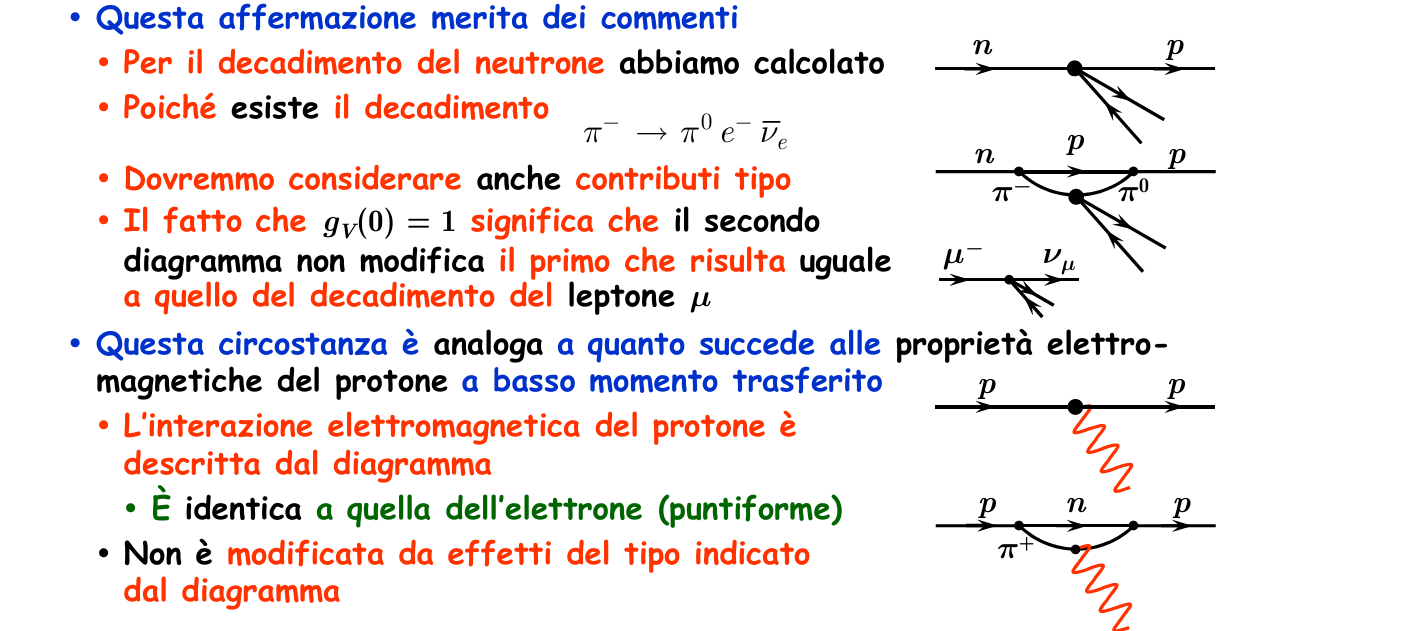
\includegraphics[width=0.9\textwidth]{Lezioni/Lezione 17/test.png}
	\label{fig:test}
\end{figure}
\section{Digressione: la corrente elettromagnetica I}
Nel caso dello scattering elastico elettrone - protone il processo è descritto dall'interazione di due correnti tramite un fotone. L'elemento di matrice della corrente leptonic si può calcolare esattamente perchè si possono usare i campi liberi
\begin{figure}[h!]
	\centering
	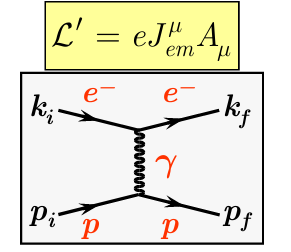
\includegraphics[width=0.4\textwidth]{Lezioni/Lezione 17/coa.png}
	\label{fig:coa}
\end{figure}
$$
J^\mu_{em} (x) = \overline{\psi}_e (x) \gamma^\mu \psi_e (x) \quad \quad \langle k_f | J^\mu_{em} (x) | k_i \rangle = \overline{u}_{k_f} \gamma^\mu u_{k_i} e^{iq \cdot x} \quad \quad q = p_f - p_i
$$
Per l'elemento di matrice della corrente adronica bisogna utilizzare una parametrizzazione simile a quanto fatto per l'interazione debole
$$
\langle p_f | J^\mu_{em} (x) | p_i \rangle = \overline{u}_{p_f} \left[ F_1 (q^2) \gamma^\mu + F_2 (q^2) \frac{i \sigma^{\mu\nu} q_\nu}{2m} + F_3 (q^2) q^\mu \right] u_{p_i} e^{iq \cdot x}
$$
Che l'interazione elettromagnetica a basso momento trasferito non sia sensibile alle interazioni forti è espresso dal fatto che
$$
F_1(0)=1
$$
La cancellazione degli effetti dovuti ai diagrammi di ordine superiore nella ridefinizione della carica elettrica (escluso la polarizzazione del vuoto) è una conseguenza della conservazione della corrente elettromagnetica
$$
\partial_\mu J^\mu_{em} (x) = 0
$$
La conservazione della corrente elettromagnetica implica anche che $F_3=0$
$$
\partial_\mu \langle p_f | J_{em}^\mu (x) | p_i \rangle = 0 \quad \quad \partial_\mu \langle p_f | J_{em}^\mu (0) | p_i \rangle e^{iq \cdot x} = q_\mu \langle p_f | J_{em}^\mu (0) | p_i \rangle = 0
$$
Imponendo questa condizione sulla parametrizzazione
$$
q_\mu \overline{u}_{p_f} \left[ F_1 (q^2) \gamma^\mu + F_2 (q^2) \frac{i \sigma^{\mu\nu} q_\nu}{2m} + F_3 (q^2) q^\mu \right] u_{p_i} = 0
$$
Osserviamo che 
$$
q_\mu \gamma^\mu = \slashed{p}_f - \slashed{p}_i
$$
Il primo termine diventa pertanto
$$
\overline{u}_{p_f} (\slashed{p}_f - \slashed{p}_i) u_{p_i} = \overline{u}_{p_f} (m_p - m_p) u_{p_i} = 0 \quad \quad \slashed{p} u_p = m u_p
$$
Il secondo termine è nullo per l'antisimmetria di $\sigma^{\mu\nu}$. Otteniamo in definitiva
$$
q_\mu \overline{u}_{p_f} F_3 (q^2) q^\mu u_{p_i} = 0 \quad \quad q^2 F_3 (q^2) \overline{u}_{p_f} u_{p_i} = 0 \quad \implies \quad F_3 (q^2) = 0
$$
L'elemento di matrice della corrente elettromagnetica del protone è pertanto
$$
\langle p_f | J_{em}^\mu (0) | p_i \rangle = \overline{u}_{p_f} \left[ F_1 (q^2) \gamma^\mu + F_2 (q^2) \frac{i \sigma^{\mu\nu} q_\nu}{2m} \right] u_{p_i}
$$
Gli esperimenti di scattering elastico $e\,\, p\to e\,\, p$ permettono di misurare i fattori di forma $F_1$ e $F_2$ in funzione del momento trasferito $q^2$.
\subsection{I fattori di forma del protone}
Alcuni risultati sui fattori di forma elettromagnetici. Le figure riportano i due fattori di forma del protone.
\begin{figure}[h!]
	\centering
	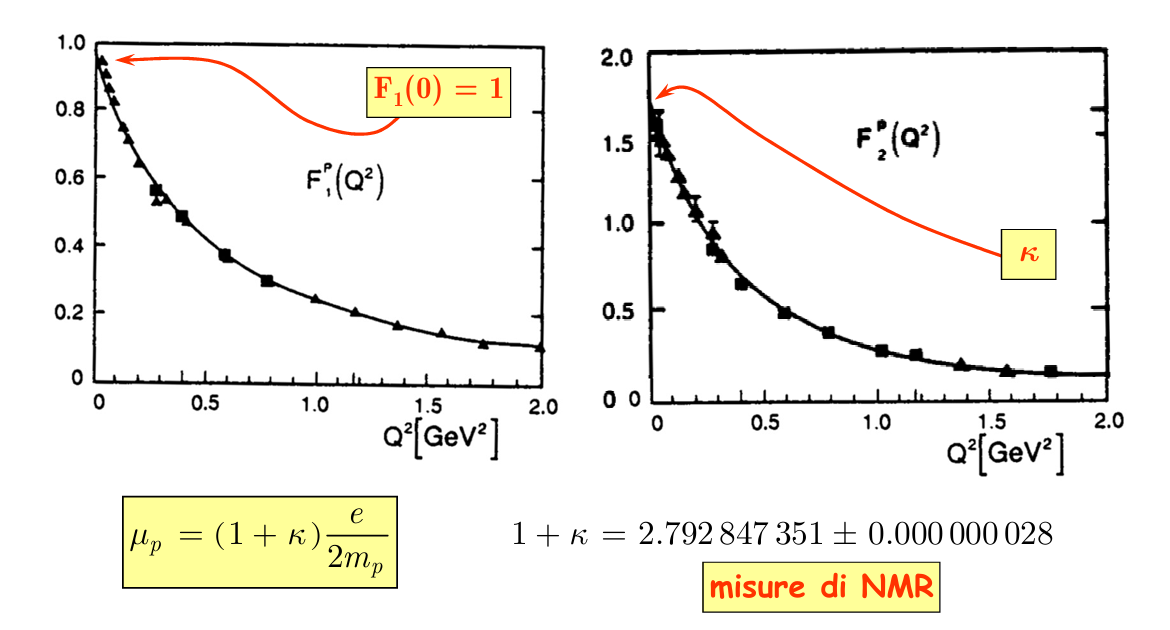
\includegraphics[width=0.8\textwidth]{Lezioni/Lezione 17/datt.png}
	\label{fig:datt}
\end{figure}
\subsection{I fattori di forma del neutrone}
Una analisi analoga può essere fatta per il neutrone
$$
\langle p_f | J_{em}^\mu (0) | p_i \rangle = \overline{u}_{p_f} \left[ F_1^n (q^2) \gamma^\mu + F_2^n (q^2) \frac{i\sigma^{\mu\nu} q_\nu}{2m} \right] u_{p_i}
$$
Le figure mostrano i risultati di esperimenti $e\,\, n\to e\,\, n$ che permettono di misurare i fattori di forma in funzione del momento trasferito $q^2$
\begin{figure}[h!]
	\centering
	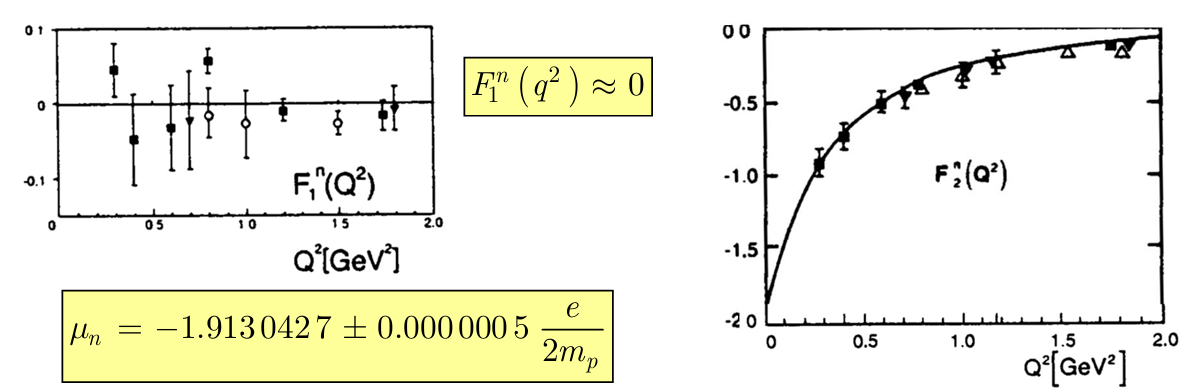
\includegraphics[width=0.8\textwidth]{Lezioni/Lezione 17/ti.png}
	\label{fig:ti}
\end{figure}
Misure dei fattori di forma del neutrone mostrano una complessa struttura di cariche e correnti. Il neutrone si composta come se avesse un nucleo positivo e una superficie negatica (con la carica totale ovviamente nulla): $n\to p+\pi^- \to n$.
\section{Digressione: la corrente elettromagnetica II}
Per una particella puntiforme che obbedisce all'equazione di Dirac:
\begin{itemize}
	\item Il Fattore di Forma $F_1$ è costante (non dipende da $q^2$) ed è uguale a $1$.
	\item Il Fattore di Forma $F_2$ è sempre nullo.
\end{itemize}
Occorre tenere presente che il fattore $F_2$ rappresenta una interazione di momento magnetico aggiuntiva. La corrente vettoriale $\overline{u}_f\gamma^\mu u_i$ contiene già una interazione di tipo magnetico. Lo abbiamo visto nel limite di bassa energia. Lo si può vedere esplicitamente con la Scomposizione di Gordon della corrente vettoriale
$$
\overline{u}_f \gamma^\mu u_i = \frac{1}{2m} \overline{u}_f \left[ (p_f + p_i)^\mu + i\sigma^{\mu\nu} (p_f - p_i)_\nu \right] u_i
$$
Dal momento che $F_2$ descrive una interazione di momento magnetico aggiuntiva viene detta "Momento Magnetico Anomalo". In particolare il suo valore a momento trasferito nullo $\kappa=F_2(0)$. In alcuni articoli o testi si fa la sostituzione $F_2\to\kappa F_2$ con $F_2(0)=1$ e $\kappa$ è il momento magnetico anomalo.
\section{Scomposizione di Gordon}
La scomposizione di Gordon mette in evidenza i due termini di interazione di una particella di Dirac
$$
\overline{u}_f \gamma^\mu u_i = \frac{1}{2m} \overline{u}_f \left[ (p_f + p_i)^\mu + i \sigma^{\mu\nu} (p_f - p_i)_\nu \right] u_i
$$
L'interazione di una particella senza spin e l'interazione dovuta al momento magnetico. Per dimostrare la relazione sviluppiamo il secondo termine
$$
\begin{aligned}
	\overline{u}_f \sigma^{\mu\nu} (p_f - p_i)_\nu u_i &= \frac{i}{2} \overline{u}_f (\gamma^\mu \gamma^\nu - \gamma^\nu \gamma^\mu) (p_f - p_i)_\nu u_i \\
	&= \frac{i}{2} \overline{u}_f (\gamma^\mu \gamma^\nu p_{f\nu} - \slashed{p}_f \gamma^\mu - \gamma^\mu \slashed{p}_i + \gamma^\nu \gamma^\mu p_{i\nu}) u_i \\
	&= -im \overline{u}_f \gamma^\mu u_i + \frac{i}{2} \overline{u}_f (\gamma^\mu \gamma^\nu p_{f\nu} + \gamma^\nu \gamma^\mu p_{i\nu}) u_i
\end{aligned}
$$
Avendo usato $\overline{u}_f \slashed{p}_f = m \overline{u}_f$ e $\slashed{p}_i u_i = m u_i$. Dalle regole di commutazione delle matrici $\gamma^\mu$
$$
\{ \gamma^\mu, \gamma^\nu \} = 2g^{\mu\nu} \to \gamma^\mu \gamma^\nu = 2g^{\mu\nu} - \gamma^\nu \gamma^\mu
$$
Utilizzando la relazione per i due termini otteniamo
$$
\begin{aligned}
	\overline{u}_f \sigma^{\mu\nu} (p_f - p_i)_\nu u_i &= -im \overline{u}_f \gamma^\mu u_i + \frac{i}{2} \overline{u}_f \left( 2g^{\mu\nu} p_{f\nu} - \gamma^\nu \gamma^\mu p_{f\nu} + 2g^{\mu\nu} p_{i\nu} - \gamma^\mu \gamma^\nu p_{i\nu} \right) u_i \\
	&= -im \overline{u}_f \gamma^\mu u_i + \frac{i}{2} \overline{u}_f \left( 2p_f^\mu - \slashed{p}_f \gamma^\mu + 2p_i^\mu - \gamma^\mu \slashed{p}_i \right) u_i
\end{aligned}
$$
Applicando ancora una volta l'equazione di Dirac otteniamo
$$
\overline{u}_f \sigma^{\mu\nu} (p_f - p_i)_\nu u_i = -i2m \overline{u}_f \gamma^\mu u_i + i \overline{u}_f (p_f^\mu + p_i^\mu) u_i
$$
Ridisponendo i termini otteniamo la scomposizione di Gordon della corrente vettoriale
$$
\overline{u}_f \gamma^\mu u_i = \frac{1}{2m} \overline{u}_f \left[ (p_f + p_i)^\mu + i\sigma^{\mu\nu} (p_f - p_i)_\nu \right] u_i
$$
Osservazione: nel caso in cui i due spinori hanno lo stesso ($p=p_i=p_f$) la formula si riduce a
$$
\overline{u}(p) \gamma^\mu u(p) = \frac{1}{2m} \overline{u}(p) \left[ (p + p)^\mu + i\sigma^{\mu\nu} (p - p)_\nu \right] u(p) = \frac{p^\mu}{m} \overline{u}(p) u(p) = 2p^\mu
$$
$$
\overline{u}(p) \gamma^\mu u(p) = 2p^\mu
$$
\section{Corrente elettromagnetica e isospin}
Il formalismo precedente può essere unificato utilizzando gli isospinori $\Psi$ per descrivere protoni e neutroni. 
$$
\Psi = \begin{pmatrix} \psi_p \\ \psi_n \end{pmatrix}
$$
Per il protone possiamo scrivere la corrente vettoriale come
$$
j_p^\mu = \overline{\psi}_p \gamma^\mu \psi_p = \begin{pmatrix} \psi_p & \psi_n \end{pmatrix} \begin{pmatrix} 1 & 0 \\ 0 & 0 \end{pmatrix} \gamma^\mu \begin{pmatrix} \psi_p \\ \psi_n \end{pmatrix}
$$
La matrice $2\times2$ può essere riscritta utilizzndo le matrici di Pauli $\tau$
$$
\begin{pmatrix} 1 & 0 \\ 0 & 0 \end{pmatrix} = \frac{1 + \tau_3}{2}
$$
Otteniamo pertanto
$$
j_p^\mu = \overline{\Psi} \gamma^\mu \frac{1 + \tau_3}{2} \Psi
$$
Occorre tenere presente che gli operatori $\gamma^\mu$ e $(1+\tau_3)/2$ operano in spazi differenti e quindi la loro posizione relativa non è essenziale. Pertanto, nello spazio dell'isospin, la corrente del protone è la somma di due termini
$$
j_p^\mu = j_S^\mu + j_3^\mu
$$
\begin{itemize}
	\item La corrente $j_S^\mu$ è un isoscalare $j_S^\mu = \overline{\Psi} \gamma^\mu 1 \Psi$ 
	\item La corrente $j_3^\mu$ è la componente $3$ dell'isovettore $\mathbf{j}_V^\mu = \frac{1}{2} \overline{\Psi} \gamma^\mu \vec{\tau} \Psi$
\end{itemize}
Analogamente per il neutrone
$$
j_n^\mu = j_S^\mu - j_3^\mu
$$
Per tutte le correnti introdotte possiamo introdurre i fattori di forma
$$
\langle p_f | j_X^\mu (0) | p_i \rangle = \overline{u}_{p_f} \left[ F_1^X (q^2) \gamma^\mu + F_2^X (q^2) \frac{i\sigma^{\mu\nu} q_\nu}{2m} \right] T u_{p_i}
$$
A seconda dei casi la corrente $J_X$, gli spinori $u$ e la matrice $T$ sono:
\begin{itemize}
	\item Per $X=n,p$ la corrente $J_X$ è un operatore nello spazio degli spinori $u_n$, $u_p$ e la matrice $T$ non è presente
	\item Per $X=S, V$ la corrente $J_X$ è anche un operatore nello spazio degli isospinori $u=(u_p, u_n)^T$ e $T$ è una delle due matrici $2\times2$
\end{itemize}
Si ha ovviamente le seguenti relazioni
$$
F_{1,2}^S = \frac{1}{2} \left( F_{1,2}^p + F_{1,2}^n \right) \quad \quad F_{1,2}^V = \frac{1}{2} \left( F_{1,2}^p - F_{1,2}^n \right)
$$
\section{Il Fattore di Forma del mesone $\pi^\pm$}
Richiamiamo alcuni risultati relativi al campo complesso $\hat{\phi}$ soluzione della equazione di Klein-Gordon. Descrive una particella puntiforme di spin zero $s^\pm$ e la corrente elettromagnetica è data da
$$
\hat{j}_{em}^\mu = ie \left[ \hat{\phi}^\dagger \partial^\mu \hat{\phi} - (\partial^\mu \hat{\phi}^\dagger) \hat{\phi} \right]
$$
Consideriamo adesso gli stati di particella singola
$$
|s^+, p\rangle = \sqrt{2E} \, \hat{a}_p^\dagger |0\rangle
$$
Utilizzando l'espansione in operatori di creazione e distruzione per il campo $\hat{\phi}$ è facile calcolare l'elemento di matrice della corrente elettromagnetica.
$$
\langle s^+, p_f \mid \hat{j}_{em}^\mu (x) \mid s^+, p_i \rangle = e \left( p_i^\mu + p_f^\mu \right) e^{-i(p_i - p_f) \cdot x}
$$
Anche nel caso del mesone $\pi$ l'interazione forte modifica l'elemento di matrice. Considerazioni di invarianza relativistica portano a concludere che l'elemento di matrice può dipendere solo dai $4-$vettori $p_i$ e $p_f$. L'elemento di matrice contiene funzioni scalari (invarianti) della variabile $q^2$. Invece che i due $4-$vettori $p_i$ e $p_f$ è conveniente utilizzare la solo somma e la loro differenza
$$
q^\mu = p_i^\mu - p_f^\mu \quad \quad P^\mu = p_i^\mu + p_f^\mu
$$
Pertanto l'elemento di matrice si può scrivere 
$$
\langle \pi^+, p_f \mid \hat{j}_{em}^\mu (x) \mid \pi^+, p_i \rangle = e \left[ F_\pi(q^2)P^\mu + G_\pi(q^2)q^\mu \right] e^{-iq \cdot x}
$$
Una ulteriore semplificazione deriva dalla conservazione della corrente elettromagnetica. Osserviamo che l'elemento di matrice dipende da $x$ solo attraverso l'esponenziale e pertanto
$$
\partial_\mu \langle f \mid \hat{j}_{em}^\mu (x) \mid i \rangle = 0 \quad \to \quad q_\mu \langle f \mid \hat{j}_{em}^\mu (x) \mid i \rangle = 0
$$
Sostituendo
$$
F_\pi(q^2) q_\mu P^\mu + G_\pi(q^2) q_\mu q^\mu = 0
$$
Si verifica facilmente che $q_\mu P^\mu=0$ e quindi
$$
q^2 G_\pi(q^2) = 0 \quad \implies \quad G_\pi(q^2) = 0
$$
In definitiva otteniamo
$$
\langle \pi^+, p_f \mid \hat{j}_{em}^\mu (x) \mid \pi^+, p_i \rangle = e F_\pi(q^2) (p_i^\mu + p_f^\mu) e^{-iq \cdot x}
$$
La funzione $F_\pi(q^2)$ è il fattore di forma elettromagnetico del pione. Per una particella scalare puntiforme $F_s(q^2)=1$
$$
\langle s^+, p_f \mid \hat{j}_{em}^\mu (x) \mid s^+, p_i \rangle = e (p_i^\mu + p_f^\mu) e^{-iq \cdot x}
$$
Il fattore di forma del $\pi^+$ si può misurare in vari modi. Mediante la fotoproduzione di pioni con fotoni reali o virtuali
$$
e^- p \to e^- n \pi^+
$$
Mediante lo scattering di pioni su elettroni
$$
\pi^- e^- \to \pi^- e^-
$$
Calcoliamo il momento trasferito $q^2$
$$
q^2 = (k_i - k_f)^2 = m_\pi^2 + m_\pi^2 - 2E_i E_f + 2\mathbf{p}_i \cdot \mathbf{p}_f
$$
In queste reazioni il momento trasferito è sempre negativo si dice che $q^2$ e space-like. Il valore massimo $q^2=0$ si ha per $\mathbf{p}_i=\mathbf{p}_f$. La figura mostra la compilazione dei dati di due esperimenti. I risultati sono compatibili con $F_\pi(0)=1$.
\begin{figure}[h!]
	\centering
	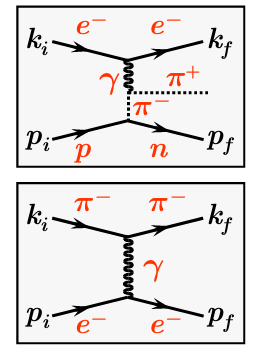
\includegraphics[width=0.2\textwidth]{Lezioni/Lezione 17/ioz1.png}
	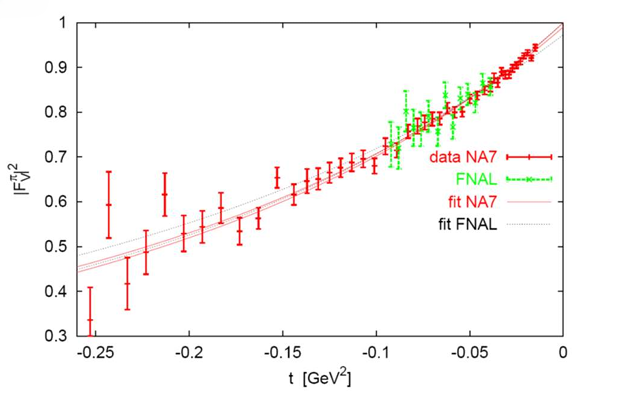
\includegraphics[width=0.6\textwidth]{Lezioni/Lezione 17/ioz2.png}
	\label{fig:ioz}
\end{figure}
\section{La corrente debole adronica}
Da quanto fin qui esposto, risulta evidente che la componente vettoriale della corrente debole adronica ha molte analogie con la componente isovettoriale della corrente elettromagnetica. Entrambe le correnti sono "insensibili" alle correzioni radiative forti. IL fattore di forma relativo tende a $1$ per $q^2\to0$. Quindi è possibile che anche la componente vettoriale della corrente debole sia conservata. Queste analogie risultano implicite se si fanno le seguenti assunzioni. Il nucleone è descritto da un campo isospinoriale. La teoria è invariante per trasformazioni globali di isospin $SU(2)$ ed esistono $3$ correnti conservate $J_1,J_2,J_3$ a cui corrispondono 3 cariche $T_1,T_2,T_3$. La componente isovettoriale della corrente adronica elettromagnetica è la corrente $J_3$
$$
j_V^\alpha = J_3^\alpha
$$
La componente vettoriale della corrente debole adronica è la corrente $J_1+iJ_2$
$$
J^{\dagger \alpha} = J_1^\alpha + i J_2^\alpha
$$
Questa ipotesi fu proposta da Gell-Mann e Feynman e prende il nome di "Conserved Vector Current" o, in breve, CVC.
\section{Il decadimento "$\beta$" del pione carico $\pi^-$}
Come applicazione della ipotesi CVC calcoliamo la larghezza del decadimento
$$
\pi^- \to \pi^0 e^- \overline{\nu}_e \quad \quad \frac{\Gamma_{\pi^- \to \pi^0 e^- \overline{\nu}_e}}{\Gamma_{\pi^- \to all}} = 1.036 \times 10^{-8}
$$
Questo è un decadimento raro dato il piccolo volume dello spazio delle fasi dovuto al piccolo $Q$ valore del decadimento. Tuttavia è molto interessante perchè consente una verifica della CVC. L'ampiezza del decadimento è data da
$$
\mathfrak{M} = \frac{G}{\sqrt{2}} \langle \pi^0 \mid J_+^\mu \mid \pi^- \rangle \overline{u}_e \gamma_\mu (1 - \gamma^5) v_\nu
$$
Dobbiamo calcolare l'elemento di matrice adronico. Innanzitutto, per l'invarianza relativistica, l'elemento di matrice può dipendere solo dai $4-$vettori $p_i$ e $p_f$
$$
\langle \pi^0 \mid J_+^\mu \mid \pi^- \rangle = a p_i^\mu + b p_f^\mu
$$
Sappiamo inoltre che la corrente ha un aparte polare e una assiale
$$
\langle \pi^0 \mid J_+^\mu \mid \pi^- \rangle = \langle \pi^0 \mid V_+^\mu \mid \pi^- \rangle + \langle \pi^0 \mid A_+^\mu \mid \pi^- \rangle
$$
Evidentemente solo $V^\mu$ si comporta come un vettore polare 
$$
\langle \pi^0 \mid A_+^\mu \mid \pi^- \rangle = 0
$$
Utilizziamo adesso l'ipotesi CVC per calcolare l'elemento di matrice
$$
\langle \pi^0 \mid J_+^\mu \mid \pi^- \rangle = \langle \pi^0 \mid V_+^\mu \mid \pi^- \rangle
$$
L'ipotesi CVC consiste nell'assumere che le correnti deboli cariche e la corrente elettromagnetica siano le tre correnti di isospin $V_1$, $V_2$, $V_3$. In particolare la componente isovettoriale della corrente elettromagnetica è $V_3$ per la corrente debole
$$
V_+ = V_1 + i V_2 \quad \quad (V_- = V_1 - i V_2)
$$
Con l'identificazione di $J=V$ abbiamo visto che le cariche $J$ e le correnti $V_i$ soddisfano le seguenti regole di commutazione
$$
[T_l, V_m^\mu] = i \varepsilon_{lmk} V_k^\mu
$$
In particolare
$$
[T_1, V_3] = i \varepsilon_{132} V_2 = -i V_2 \quad \quad [T_2, V_3] = i \varepsilon_{231} V_1 = i V_1
$$
Dalle due relazioni precedenti si ottiene
$$
[T_1, V_3] + i[T_2, V_3] = -iV_2 - V_1 = -V_+ = [T_1 + iT_2, V_3] = [T_+, V_3]
$$
In conclusione
$$
[V_3, T_+] = V_+
$$
Questa regola ci permette di trovare una relazione fra l'elemento di matrice del decadimento $\beta$ del $\pi^-$ e l'elemento di matrice della corrente elettromagnetica del $\pi^-$. Il $\pi^-$ e il $\pi^0$ sono due autostati $|T,T_3\rangle$ dell'isospin.
$$
|\pi^-\rangle = |1, -1\rangle \quad \quad |\pi^0\rangle = |1, 0\rangle
$$
Otteniamo pertanto
$$
\langle \pi^0 \mid V_+^\mu \mid \pi^- \rangle = \langle 1, 0 \mid V_+^\mu \mid 1, -1 \rangle = \langle 1, 0 \mid [V_3, T_+] \mid 1, -1 \rangle
$$
$$
= \langle 1, 0 \mid V_3 T_+ - T_+ V_3 \mid 1, -1 \rangle = \langle 1, 0 \mid V_3 T_+ \mid 1, -1 \rangle - \langle 1, 0 \mid T_+ V_3 \mid 1, -1 \rangle
$$
Sfruttiamo le proprietà degli operatori di innalzamento e abbassamento
$$
T_+ |T, T_3\rangle = \sqrt{(T - T_3)(T + T_3 + 1)} |T, T_3 + 1\rangle \quad \quad T_+ |1, -1\rangle = \sqrt{2} |1, 0\rangle
$$
$$
T_- |T, T_3\rangle = \sqrt{(T + T_3)(T - T_3 + 1)} |T, T_3 - 1\rangle \quad \quad T_- |1, 0\rangle = \sqrt{2} |1, -1\rangle
$$
Introducendo nell'elemento di matrice
$$
\langle 1, 0 \mid V_3 T_+ \mid 1, -1 \rangle - \langle 1, 0 \mid T_+ V_3 \mid 1, -1 \rangle = \sqrt{2} \langle 1, 0 \mid V_3 \mid 1, 0 \rangle - \sqrt{2} \langle 1, -1 \mid V_3 \mid 1, -1 \rangle
$$
Utilizzando l'ipotesi CVC abbiamo pertanto ottenuto
$$
\langle \pi^0 \mid V_+^\mu \mid \pi^- \rangle = \sqrt{2} \langle \pi^0 \mid V_3 \mid \pi^0 \rangle - \sqrt{2} \langle \pi^- \mid V_3 \mid \pi^- \rangle
$$
Ricordiamo inoltre che l'ipotesi CVC identifica $V_3$ con la corrente elettromagnetica $j_{em}$. Un'ultima semplificazione si ottiene dalla proprietà della corrente elettromagnetica rispetto all'operatore di coniugazione di carica $C=C^{-1}=C^\dagger$
$$
C^{-1} j_{\text{em}}^\mu C = - j_{\text{em}}^\mu
$$
Questa relazione dice semplicemente che il segno del campo elettromagnetico dipende dal segno della carica elettrica della particella. Inoltre il $\pi^0$ è un autostato di $C$ con autovalore $+1$ $C|\pi^0\rangle=+|\pi^0\rangle$. Otteniamo pertanto
$$
\langle \pi^0 \mid j_{\text{em}}^\mu \mid \pi^0 \rangle = \langle \pi^0 \mid C^\dagger j_{\text{em}}^\mu C \mid \pi^0 \rangle = - \langle \pi^0 \mid j_{\text{em}}^\mu \mid \pi^0 \rangle
$$
Da cui
$$
\langle \pi^0 \mid j_{\text{em}}^\mu \mid \pi^0 \rangle = 0
$$
Pertanto l'elemento di matrice del decadimento $\beta$ del $\pi^-$ è
$$
\langle \pi^0 \mid V_+^\mu \mid \pi^- \rangle = -\sqrt{2} \langle \pi^- \mid j_{\text{em}}^\mu \mid \pi^- \rangle
$$
Pertanto che l'elemento di matrice adronico della corrente debole può essere calcolato a partire dall'elemento di matrice della corrente elettromagnetica
$$
\langle \pi^\pm, p_f \mid j_{\text{em}}^\mu (0) \mid \pi^\pm, p_i \rangle = F_\pi (q^2) (p_i^\mu + p_f^\mu)
$$
Il $Q$ valore del decadimento è molto piccolo
$$
Q = m_{\pi^-} - m_{\pi^0} - m_e = 139.570 - 134.977 - 0.511 = 4.082 \text{ MeV}
$$
La massima quantità di moto è di appena $4\,\unit{MeV}$ ($\mathbf{p}_i=0$)
$$
q_{\text{max}}^2 = m_{\pi^-}^2 + m_{\pi^0}^2 - 2E_i E_f + 2\mathbf{p}_i \cdot \mathbf{p}_f = m_{\pi^-}^2 + m_{\pi^0}^2 - 2m_{\pi^-} E_{\pi^0}
$$
Introducendo i valori numerici vediamo che $q^2\approx(m_{\pi^-}-m_{\pi^0})^2$ con $(E_{\pi^0}\approx m_{\pi^0})$
$$
q_{\text{max}}^2 = 4.626 \text{ MeV}^2 = 4.626 \times 10^{-6} \text{ GeV}^2 \simeq 0
$$
Quindi è possibile trascurare la dipendenza da $q^2$ e assumere $F_\pi(q^2)=1$ pertanto
$$
\langle \pi^0 \mid V_+^\mu \mid \pi^- \rangle = -\sqrt{2} (p_i^\mu + p_f^\mu)
$$
Il calcolo è a questo punto semplice e lasciato come esercizio
$$
\Gamma_{\pi^0 e \nu} = \frac{G_\beta^2}{30\pi^3} (m_{\pi^-} - m_{\pi^0})^5
$$
Da confrontare con
$$
\Gamma_{l\nu} = \frac{G_\beta^2}{8\pi} f_\pi^2 m_l^2 m_\pi \left( 1 - \frac{m_l^2}{m_\pi^2} \right)^2
$$
\section{Il decadimento $\beta$ del neutrone}
Con lo stesso procedimento nel caso del decadimento $\beta$ del neutrone si può verificare la relazione fra la parte vettoriale dell'elemento di matrice della corrente carica e la parte isovettoriale della corrente elettromagnetica. Infatti per l'ipotesi CVC
$$
\langle p \mid J_+^\mu \mid n \rangle = \langle p \mid V_+^\mu \mid n \rangle = \langle \frac{1}{2}, \frac{1}{2} \mid V_+^\mu \mid \frac{1}{2}, -\frac{1}{2} \rangle
$$
Utilizzando il commutatore
$$
[V_3, T_+] = V_+
$$
Otteniamo
$$
\langle \frac{1}{2}, \frac{1}{2} \mid V_+^\mu \mid \frac{1}{2}, -\frac{1}{2} \rangle = \langle \frac{1}{2}, \frac{1}{2} \mid V_3 T_+ - T_+ V_3 \mid \frac{1}{2}, -\frac{1}{2} \rangle
$$
Per le proprietà di $T_+$ e $T_-$
$$
T_+ \left| \frac{1}{2}, -\frac{1}{2} \right\rangle = \left| \frac{1}{2}, +\frac{1}{2} \right\rangle \quad \quad T_- \left| \frac{1}{2}, \frac{1}{2} \right\rangle = \left| \frac{1}{2}, -\frac{1}{2} \right\rangle
$$
Introduciamo nell'elemento di matrice
$$
\langle \frac{1}{2}, \frac{1}{2} \mid V_+^\mu \mid \frac{1}{2}, -\frac{1}{2} \rangle = \langle \frac{1}{2}, \frac{1}{2} \mid V_3 \mid \frac{1}{2}, \frac{1}{2} \rangle - \langle \frac{1}{2}, -\frac{1}{2} \mid V_3 \mid \frac{1}{2}, -\frac{1}{2} \rangle
$$
Abbiamo pertanto la relazione fra l'elemento di matrice del decadimento $\beta$ e quello della corrente isovettoriale elettromagnetica
$$
\langle p \mid V_+^\mu \mid n \rangle = \langle p \mid j_{\text{em}}^\mu \mid p \rangle - \langle n \mid j_{\text{em}}^\mu \mid n \rangle
$$